


% Latex Quelldatei zur Bachelorarbeit

%\documentclass{scrartcl}

\documentclass[
	12pt,
	halfparskip,
	%parskip,
	a4paper,
	%oneside,
	%ngerman,
	%noonelinecaption,
	abstract,
	bibliography=totoc,
	liststotoc
]{scrreprt}

%\documentclass{scrbook}

%\usepackage[ngerman]{babel}
\usepackage{ngerman}
%\usepackage{citep}
\usepackage{natbib}
\usepackage[utf8]{inputenc}
\usepackage{graphicx}
%\usepackage[T1]{fontenc}
\usepackage{hyperref}
%\usepackage{tabularx}

\hypersetup{
	pdfauthor = {Murat Akgül},
	pdftitle = {Kamisado},
	pdfsubject = {Proposal zur Bachelorarbeit},
	pdfkeywords = {Bachelor, Kamisado, Alpha, Beta, Suche, Minimax, 				künstliche, Intelligenz, Java, Brettspiel},
	pdfcreator = {Murat Akgül},
	pdfproducer = {Murat Akgül}
}

\begin{document}

\bibliographystyle{dinat}

%\citestyle{dinat}

\graphicspath{{bilder/}}

\titlehead{Technische Universität Berlin
	\\ Fakultät Elektrotechnik und Informatik
	\\ Institut für Softwaretechnik und Theoretische Informatik
	\\ Fachgebiet Künstliche Intelligenz
}
\subject{Proposal zur Bachelorarbeit}
\title{Kamisado - Brettspiel in Java}
\subtitle{Strategisches 2-Personen Nullsummenspiel mit perfekter Information}
\author{Murat Akgül
	\\ Matrikelnr.: 221131
	\\ E-Mail: osbornx22@gmail.com}
\date{\today}
\publishers{Betreut von Dr.- Ing. Stefan Fricke
	\\ E-Mail: stefan.fricke@dai-labor.de}

\maketitle

\begin{abstract}

Kamisado ist ein “Schach-artiges” Brettspiel. Bei dieser Arbeit geht es um die Umsetzung als Computerspiel, welches in Java programmiert wird. Es werden entweder zwei Personen an einem Computer gegeneinander oder ein Spieler gegen den Computer spielen können. Dabei geht es hauptsächlich um die künstliche Intelligenz. Da es sich um ein strategisches 2-Personen Nullsummenspiel handelt, wird mittels Alpha-Beta-Suche der beste Zug ermittelt und ausgeführt. Außerdem wird durch iterative Tiefensuche gewährleistet, dass die Berechnungen in angemesser Zeit abgeschlossen werden.

\end{abstract}

\tableofcontents

\chapter{Einleitung}

In diesem Einführungskapitel werden die Zielstellung und die dazugehörige wissenschaftliche Fragestellung erläutert.

\section{Zielstellung}

Das Ziel dieser Arbeit ist die Umsetzung des Brettspiels Kamisado in ein selbstständig ausführbares Java-Programm. Ein wichtiger Teil dieser Arbeit ist die Implementierung der künstlichen Intelligenz, welche aus vorhandenen Entwicklungsmustern übernommen und in diesem konkreten Fall angepasst werden muss.

Bei der Implementierung der Alpha-Beta-Suche stellt die Bewertungsfunktion für Spielsituationen eine große Rolle und besondere Herausforderung dar, da diese für jedes Spiel speziell entwickelt werden muss und dazu ein großes Spektrum an Möglichkeiten zur Auswahl steht.

\section{Wissenschaftliche Fragestellung}

Aus wissenschaftlicher Sicht ist klarzustellen, ob die gewählten Algorithmen korrekt und optimal für Kamisado sind, also ob das Spiel die Voraussetzungen erfüllt, die zur Anwendung der ausgewählten Entwicklungsmuster nötig sind. Desweiteren muss klargestellt werden, wie zu überprüfen ist, ob diese Algorithmen korrekt umgesetzt und angepasst wurden oder ob es noch Verbesserungspotenziale gibt.

Im besonderen ist herauszustellen, ob die Komplexität der Bewertungsfunktion in akzeptablen Grenzen liegt und wieviel Verbesserungspotenzial theoretisch noch auszuschöpfen wäre. Dazu ist zu klären, ob die gewählten Datenstrukturen optimal gewählt und implementiert sind oder ob es noch andere, eventuell bessere Möglichkeiten gibt, da diese einen besonderen Einfluss auf die Komplexität der Bewertungsfunktion haben.

\chapter{Kamisado}

Kamisado ist ein abstraktes Brettspiel. Es wurde von im Jahre 2009 von Peter Burley entwickelt und vom Verlag HUCH \& friends veröffentlicht. Kamisdo ist ein strategisches 2-Personen-Spiel und eine normale Partie dauert 20 bis 30 Minuten. \citep{spieletest}

\begin{figure}[htb]
\begin{center}
\fbox{
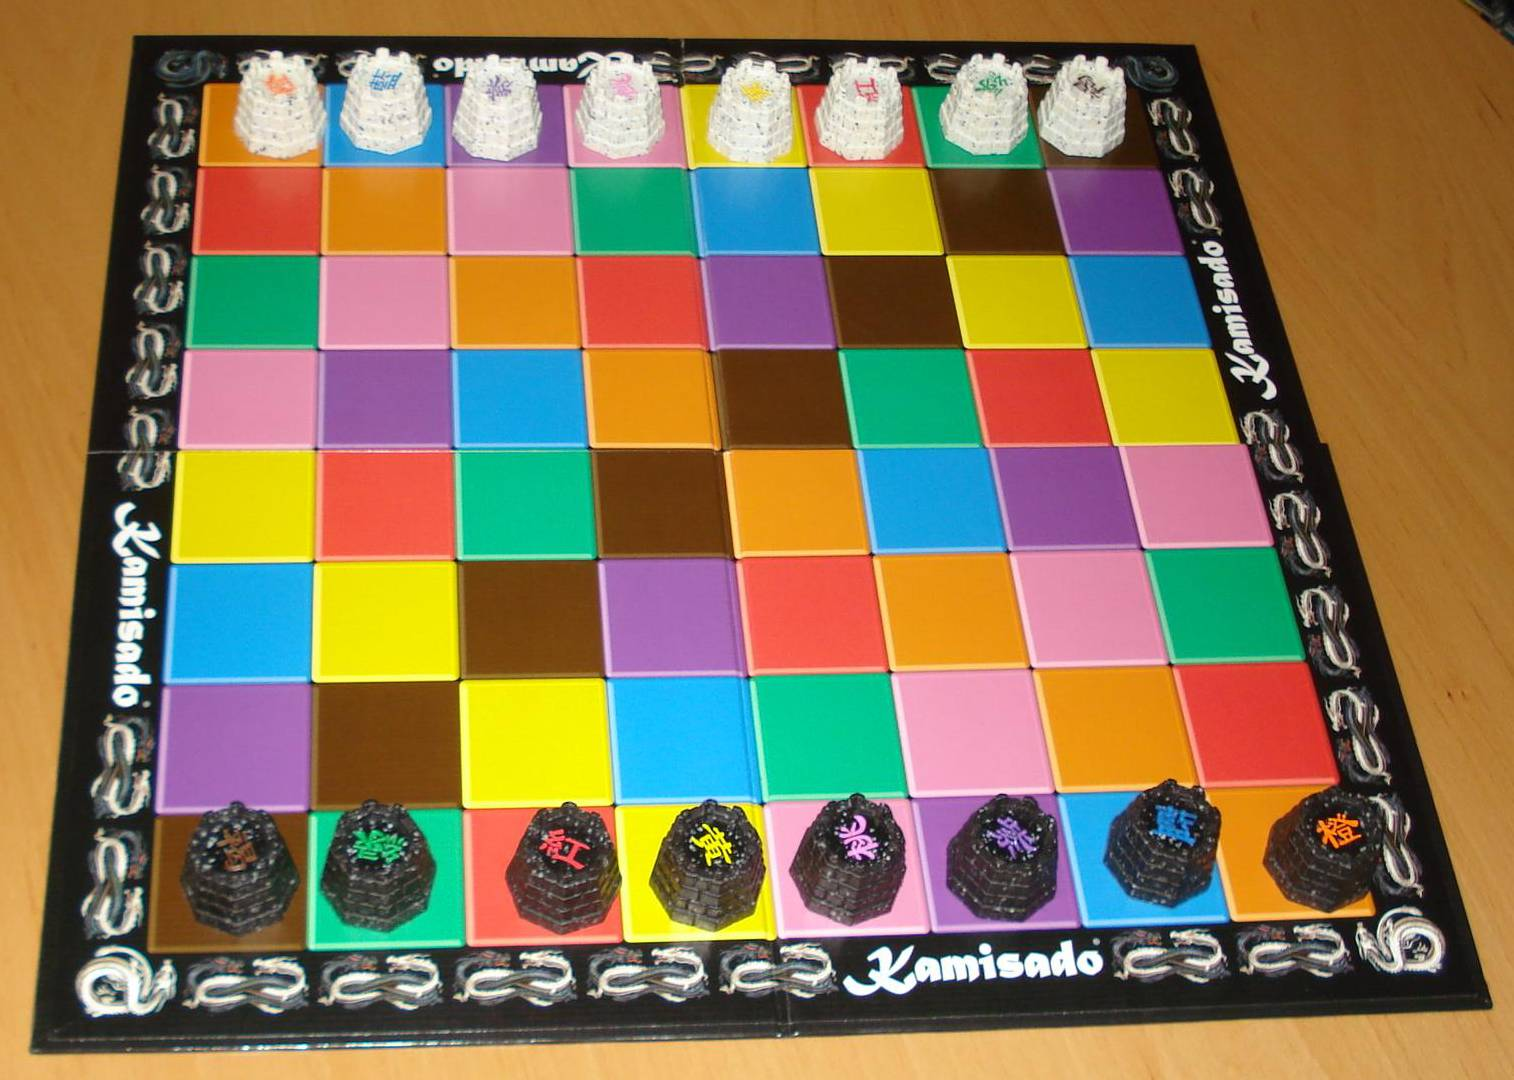
\includegraphics[width=0.9\textwidth]{startspiel.jpg}
}
\end{center}
\caption{Der Aufbau zu Beginn des Spiels \citep{4players}.}
\label{fig:startspiel}
\end{figure}

\section{Aufbau}

Das Spielfeld besteht aus 8 mal 8 Feldern. Jedes Feld hat eine bestimmte Farbe, wobei es insgesamt nur 8 verschiedene Farben im Spiel gibt: Braun, Grün, Rot, Gelb, Rosa, Lila, Blau und Orange. Jeder Spieler hat 8 Figuren, die in der Grundfarbe weiß oder schwarz sind, allerdings zusätzlich mit einer der 8 Farben markiert sind. Die Figuren werden wie in Abbildung~\ref{fig:startspiel} an der Grundlinie der Farbe entsprechend aufgestellt. \citep{huch}

\section{Grundlregeln der Einzelpartie}

Bei der ersten Partie fängt der schwarze Spieler an, in allen folgenden Partien der jeweilige verlierer der vorherigen Partie. Die Figuren werden nun abwechselnd und nacheinander bewegt. Es darf immer nur die Figur mit der Farbe bewegt werden, welche der Feldfarbe entspricht, die der Gegner mit seinem letzten Zug erreicht hat. Dabei sind nur diagonale oder gerade Bewegungen in die Richtung der gegnerischen Grundlinie gestattet. Seitliche- oder Rückwärts-Bewegungen sind nicht gestattet. Beim ersten Zug darf der Spieler der anfängt eine beliebige Farbe auswählen. \citep{kamisado.com}

\begin{figure}[htb]
\begin{center}
\fbox{
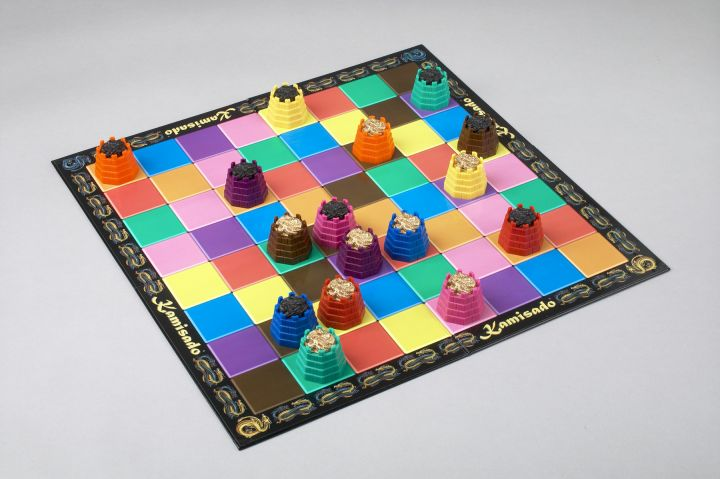
\includegraphics[width=0.9\textwidth]{mittelspiel.jpg}
}
\end{center}
\caption{Eine Beispielhafte Aufstellung im Verlauf eines Spiels
\citep{kamisado.com}.}
\label{fig:mittelspiel}
\end{figure}

\section{Ziel und Sieg}

Ziel des Spiels ist es mit einer eigenen Figur auf die gegnerische Grundlinie zu kommen. Dazu muss der Gegner vorher eine Bewegung auf ein Feld mit einer Farbe machen, sodass danach eine Bewegung der entsprechenden eigenen Figur auf die gegnerische Grundlinie möglich ist. Es gibt noch weitere Varianten dieses Spiel, allerdings wird darauf in dieser Arbeit nicht eingegangen. \citep{huch}

\chapter{Grundbegriffe der Spieltheorie}

Die Spieltheorie war ursprünglich ein Teilgebiet der Mathematik, allerdings haben sich die Anwendungsbereiche auf Informatik, Psychologie, Wirtschaft und Andere ausgeweitet. In der Spieltheorie geht “es um die angemesse Beschreibung und Modellierung von Entscheidungssituationen bzw. Spielen” \citep[S. 2]{wiese}.

\section{Nullsummenspiel}

Bei einem Nullsummenspiel im Sinne der Spieltheorie handelt es sich um ein Spiel, bei dem die Summe aller Einzahlungen der Summe aller Auszahlungen entspricht, also der Gewinn des einen Spielers ebenso der Verlust des anderen Spielers ist. \citep[S. 406]{strat}

Diese Eigenschaft trifft für Kamisado zu, weil immer genau einer der beiden Spieler gewinnt (+1) und der andere Verliert (-1). Die Summe der Gewinne und Verluste (+1 + -1 = 0) beträgt also Null.

\section{Perfekte Information}

Ein Spiel mit perfekter Information im Sinne der Spieltheorie ist ein Spiel in dem es keinerlei zufällige Elemente gibt und jedem Spieler alle ausgeführten Züge bekannt sind. Es darf auch keine verdeckten Karten oder ähnliches geben. Jedes Spiel mit perfekten Informationen ist auch Spiel mit vollständigen Informationen, da diese lediglich verlangen, dass es keine unquantifizierbaren Zufallselemete gibt. \citep[S. 65]{info}

Bei Kamisado gibt es keine Würfel oder andere Zufallselemente. Das Spielfeld ist fest bestimmt und jedem gänzlich bekannt. Jede Figur und Zugmöglichkeit inkl. Regeln sind ebenso beiden Spielern bekannt. Kamisado ist ein Spiel mit perfekter Information.

% \section{Strategiespiel}

\chapter{Algorithmen der künstliche Intelligenz}

Zum Aufbau einer künstlichen Intelligenz wurden bereits bestimmte mathematisch korrekte Entwurfsmuster entwickelt, die je nach Anforderung und Situation auszuwählen sind. Da Kamisado ein Nullsummenspiel mit perfekter Information ist, werden die dafür in Frage kommen Entwurfsmuster vorgestellt.

\section{Minimax-Algorithmus}

Mit dem Minimax-Algorithmus lassen sich optimale Züge bzw. die optimale Strategie für bestimmte Spiele finden. Insbesondere für strategische 2-Personen Nullsummenspiele mit perfekten Informationen ist der Algorithmus optimal und vollständig, allerdings ist die Vollständigkeit in der Praxis nicht immer erreichbar. \citep[S. 161]{ai}

Bei diesem Algorithmus, welche einer Tiefensuche entspricht, wird stets der minimal zu erwartende Gewinn maximiert bzw. der maximal zu erwartende Verlust minimiert. Dazu wird ein Suchbaum aufgestellt, wobei die Ebenen abwechselnd einen Zug der ersten und dann des zweiten Spieler darstellen. Zu jedem Zug des Spielers (Elternknoten) werden die darauf möglichen gegnerischen Folgezüge generiert (Kinderknoten). Mithilfe einer Bewertungsfunktion kann beurteilt werden, wie gut oder schlecht ein jeweiliger Pfad ist und somit kann der beste Zug für jede Spielsituation ausgewählt werden. \citep{vl}

Es sind also mindestens zwei Hilfsfunktionen nötig, einmal ein Zuggenerator, der regelgerechte Folgezüge generiert, um daraus mögliche Folgesituationen zu ermitteln. Solch ein Zuggenerator sollte relativ einfach zu implementieren sein. Allerdings ist dies bei der Bewertungsfunktion etwas komplizierter, da es verschiedene Möglichkeiten gibt, um einer Situation im Spiel einen nummerischen Wert zuzuteilen, aus dem im Vergleich zu anderen Situationen ein Vorteil oder Nachteil zu ermitteln ist. Dazu wird in der Regel eine Linearkombination aus verschiedenen Eigenschaften der jeweiligen Spielsituation gebildet. Außerdem ist noch eine Funktion nötig, die Sieg, Remi oder Verlustsituationen erkennt. \citep[S. 162f]{ai}

Wie schon kurz erwähnt, ist die Vollständigkeit nicht immer realisierbar. Dies kann aus der größe des Baumes resultieren, also aus einem hohen Verzweigungsgrad und/oder einer hohen Baumtiefe. Sei b der Verzweigungsfaktor und m die Baumtiefe, dann beträgt die Zeitkomplexität vom Minimax-Algorithmus $O(b^m)$. Der Zeitaufwand steigt also für komplexere Spiele sehr stark an, deswegen ist ein leicht erweiterter Algorithmus für solche Fälle besser geeignet, nämlich die Alpha-Beta-Suche. \citep{vl, minimax}

\section{Alpha-Beta-Suche}

Der grundlegende Unterschied der Alpha-Beta-Suche zum Minimax-Algorithmus besteht darin, dass nun nicht der ganze Suchbaum aufgespannt wird, sondern nur diejenigen Pfade berechnet werden, die das Endergebnis überhaupt noch beeinflussen können. Bei einem MIN-Knoten wird dies auch Alpha-Cutoff genannt und bei einem MAX-Knoten Beta-Cutoff. Bei optimaler Reihenfolge der Züge, die zuerst berechnet werden, beträgt der Zeitaufwand nur noch $O(b^{m/2})$. \citep{vl}

Mithilfer der Bewertungsfunktion können die zu berechnenden Folgesituationen vorsortiert werden. So können eventuell besonders vorteilhafte Züge vor den wahrscheinlich schlechteren Zügen berechnet werden, wodurch die schlechteren durch einen Cutoff wegfallen können, ohne viel Rechenzeit investiert zu haben. \citep[S. 169]{ai} 

\chapter{Aufgabenstellung und Lösungsansatz}

Als Teile dieser Bachelorarbeit werden ein ausführbares Programm und eine schriftliche Ausarbeitung verlangt. Zum Abschluss wird diese Arbeit noch verteidigt werden müssen.

\begin{figure}[htb]
\begin{center}
\fbox{
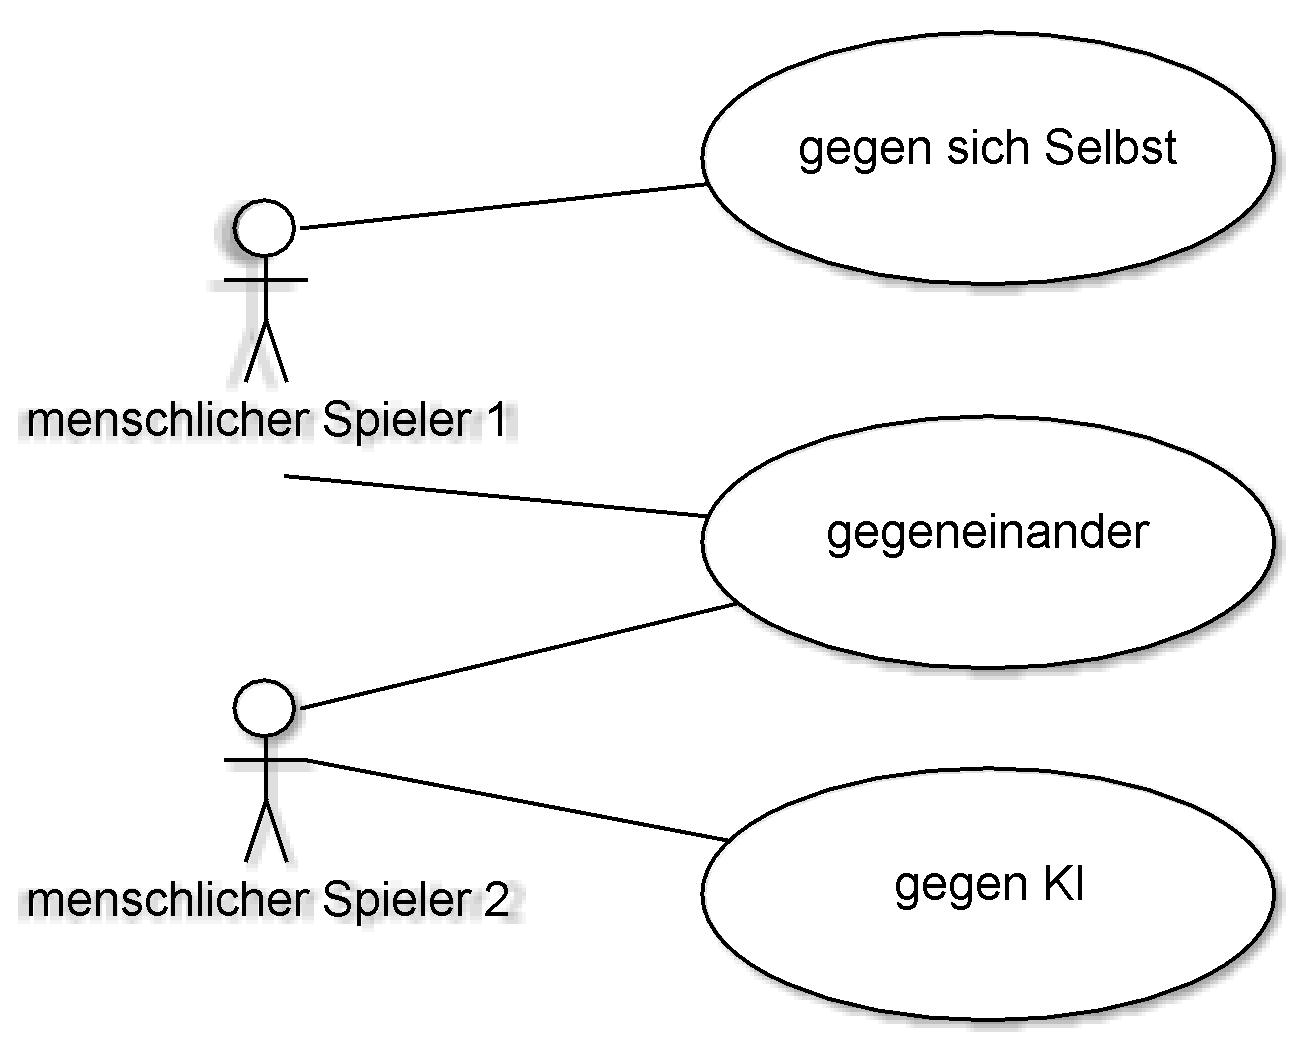
\includegraphics[width=0.6\textwidth]{usecase.png}
}
\end{center}
\caption{Ein Anwendungsfalldiagramm mit den Fällen, die umgesetzt werden müssen.}
\label{fig:usecase}
\end{figure}

\section{Anforderung aus der Aufgabenstellung}

Bei dem ausführbaren Programm, handelt es sich um die Implementation von Kamisado. Dazu gehört zunächst eine grafische Benutzeroberfläche zur Darstellung des Spiels und der Interaktion mit dem Nutzer oder den Nutzern. Dabei soll es möglich sein, gegen sich Selbst, gegen einen anderen Spieler am gleichen Computer oder den Computer selbst zu spielen (siehe Abbildung~\ref{fig:usecase}). Der Computer bedient sich dabei einer künstlichen Intelligenz, dessen Strategie auf der Alpha-Beta-Suche mit iterativer Tiefensuche basiert. Es dürfen nur regelgerechte Züge ausgeführt werden und es wird automatisch der Sieger bzw. Verlierer erkannt.


\section{Vorgehensmodell zur Entwicklung}

Als ersten Schritt im Prozess zur Lösung dieser Aufgabe muss ein Vorgehensmodell aus der Softwareentwicklung ausgewählt werden. Hierfür ist aufgrund der charakteristischen Eigenschaften während der Entwicklung einer Bachelorarbeit das Spiralmodell gut geeignet. Dies ergibt sich daraus, dass eine Version gefertigt wird und entsprechend der Kritik des Betreuers eine Weiterentwicklung stattfindet. Wie in Abbildung~\ref{fig:spiralmodell} dargestellt, kann dieses Proposal als “Planung der Anforderungen” angesehen werden, darauf folgt ein “Entwicklungplan”, der auch schon in diesem Proposal zumindest Teilweise stattfindet und danach folgen verschiedene “Entwurfs”-phasen mit “Testplanungen” und “Tests”, welche auch schon parallel zur Ausarbeitung dieses Proposals begonnen wurden. \citep{spiral}

\begin{figure}[htb]
\begin{center}
\fbox{
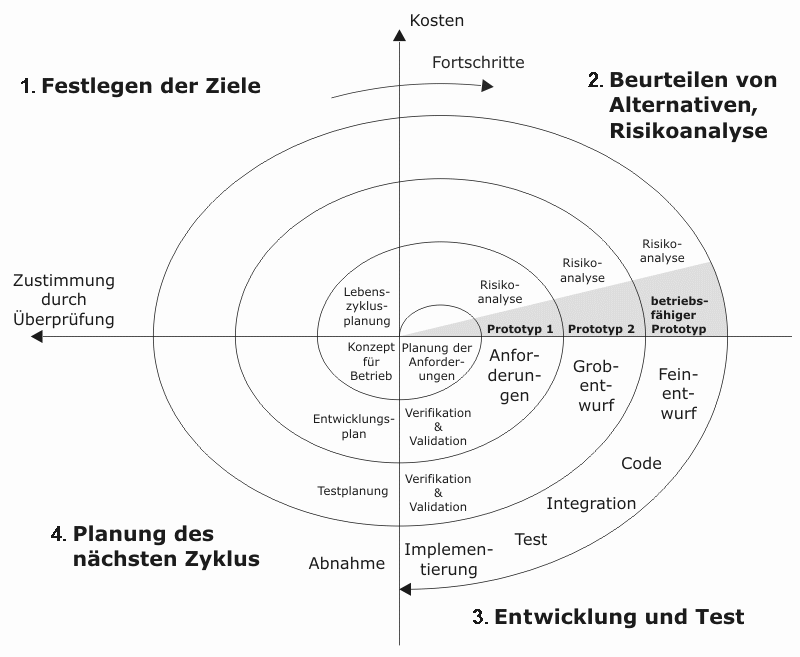
\includegraphics[width=0.7\textwidth]{spiralmodell.png}
}
\end{center}
\caption{Die Phasen der Softwareentwicklung nach dem Spiralmodell. \citep{conny}}
\label{fig:spiralmodell}
\end{figure}

\section{Klassendiagramm zum Gesamtprojekt}

Da Java eine objektorientierte Programmiersprache ist, wurde zunächst eine intuitiv entsprechende Klassenmodellierung gewählt.

\begin{samepage}
Die Objekte des Spiels sind schnell aufgezählt:
\begin{itemize}
\item Das Spielfeld besteht aus 64 Feldern.
\item Es gibt 16 Figuren, die
\begin{itemize}
\item einem Spieler gehören,
\item eine Grundfarbe und
\item eine Zusatzfarbe haben.
\end{itemize}
\end{itemize}
\end{samepage}

So lässt sich ganz einfach ein Klassendiagramm (siehe Abbildung~\ref{fig:klassendiagramm}) mit den entpsrechenden Kardinalitäten, Assoziationen und Aggregationen aufbauen.

\begin{figure}[htb]
\begin{center}
\fbox{
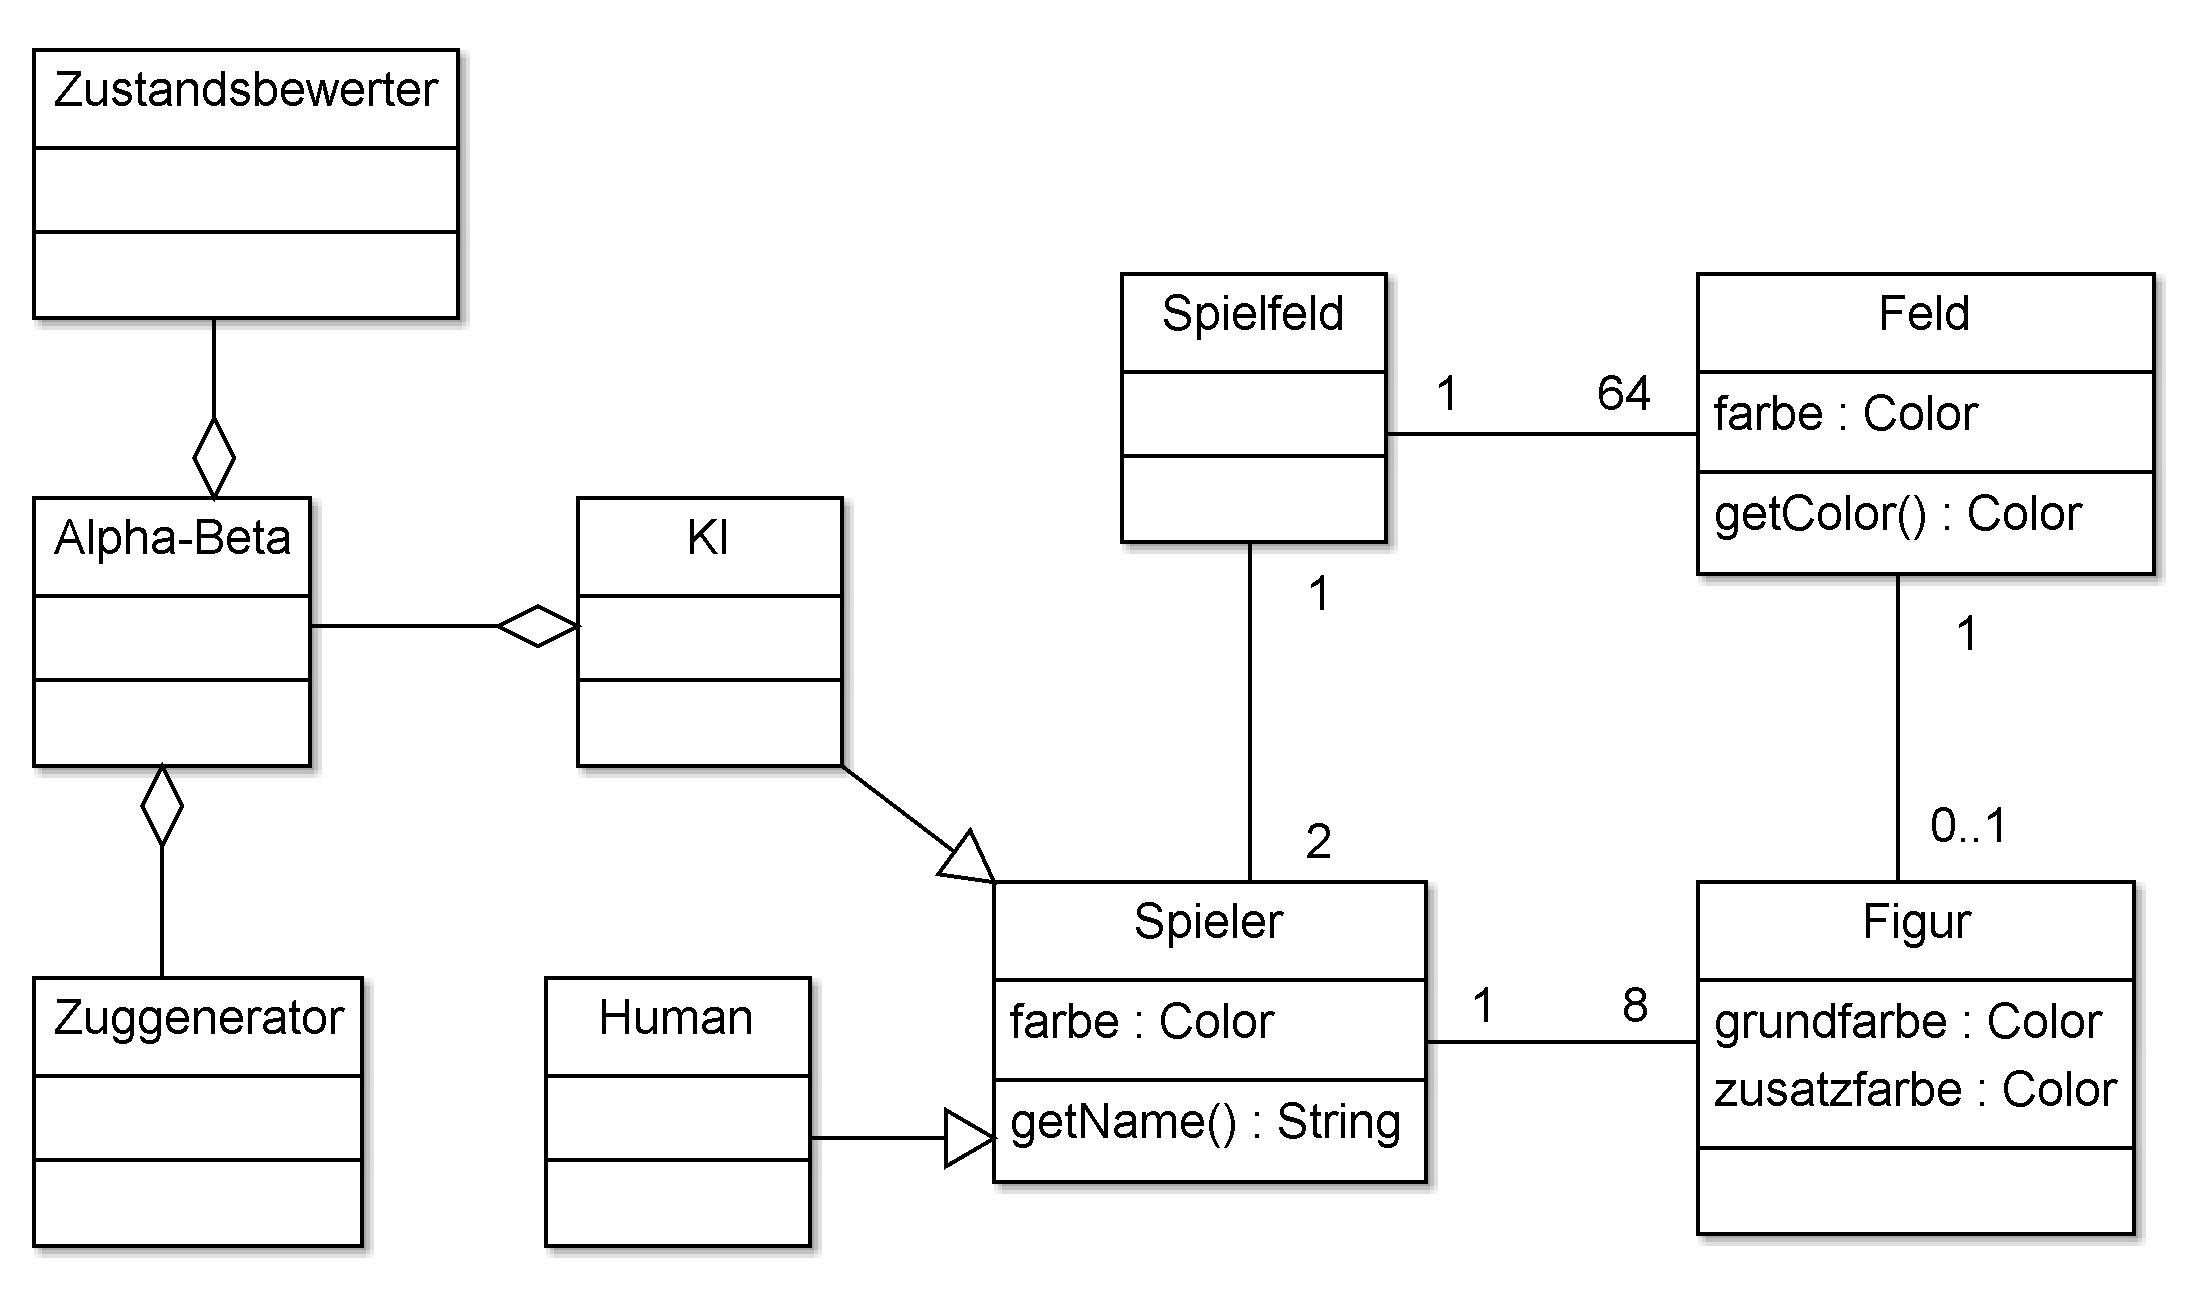
\includegraphics[width=0.8\textwidth]{klassendiagramm.png}
}
\end{center}
\caption{Ein Klassendiagramm zu Kamisado mit Objekten, Methoden und Attributen.}
\label{fig:klassendiagramm}
\end{figure}

\section{Aktivitätsdiagramm zu Ausführung eines Zuges}

Um die Funktionsweise des Programms etwas besser verstehen zu können, ist in Abbildung~\ref{fig:aktiv} ein Aktivitätsdiagramm zur Ausführung eines Zuges im Laufe des Spiels dargestellt.

\begin{figure}[htb]
\begin{center}
\fbox{
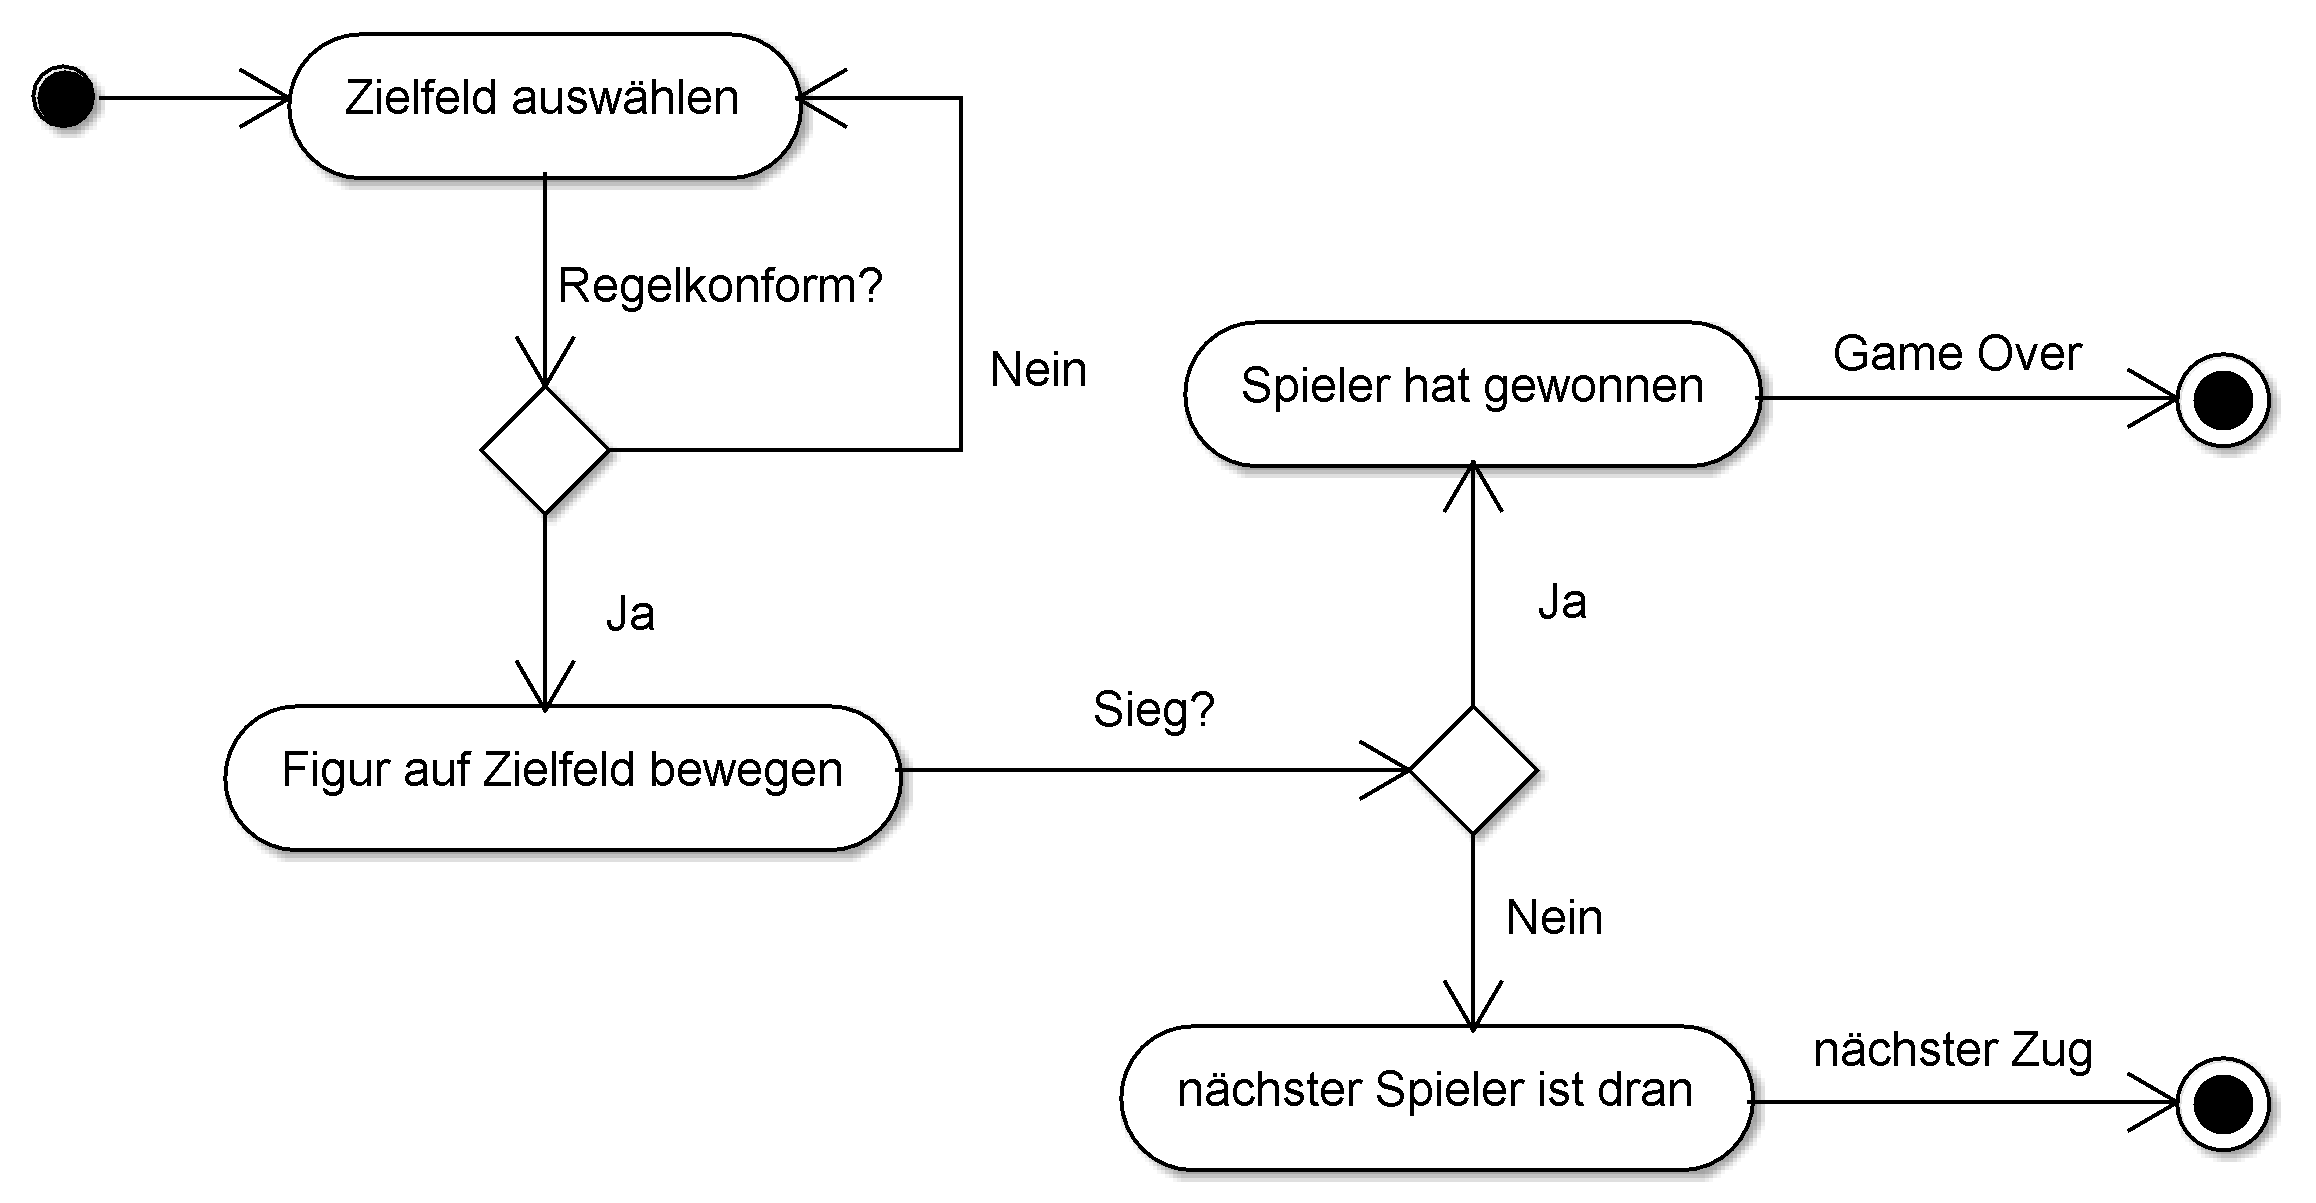
\includegraphics[width=0.8\textwidth]{aktiv.png}
}
\end{center}
\caption{Aktivitätsdiagramm zur Ausführung eines Zuges von einem Spieler im Laufe eines Spiels.}
\label{fig:aktiv}
\end{figure}

Abgesehen vom ersten Zug, ist in allen nachfolgenden Zügen eindeutig bestimmt, welche Figur der Spieler bewegen muss, da dies von der Zielfeldfarbe des vorherigen Zuges vom Gegner äbhängt. Deswegen soll der Spieler einfach nur das “Zielfeld auswählen”. Falls das Zielfeld mit der jeweiligen Figur “regelkonform” erreichbar ist, dann wird die “Figur auf das Zielfeld bewegt”, andernfalls muss der Spieler ein neues “Zielfeld auswählen”. Falls durch diesen Zug der “Spieler gewonnen hat”, dann ist das Spiel vorbei (Game Over), andernfalls ist der “nächste Spieler dran”. Diese Aktivität wird solange wiederholt bis ein Sieger feststeht (Game Over).

\section{Überlegungen zur Bewertungsfunktion}

Wie bereits erwähnt, ist die Bewertungsfunktion ein entscheidender Teil der Alpha-Beta-Suche und somit auch wichtig für die Stärke der künstlichen Intelligenz. Zur Ermittlung einer guten Bewertungsfuntkion werden einige Versuche und Tests nötig sein. Dazu könnten auch verschiedene Bewertungsfunktion gegeneinander spielen, um deren jeweilige Stärke zu ermitteln.

\begin{samepage}
Zunächst ist es wichtig zu wissen, welche Kriterien zur Aufstellung einer Bewertungsfunktion überhaupt zur Verfügung stehen, wobei zu unterscheiden ist, welcher Spieler gerade dran ist:
\begin{itemize}
\item Anzahl der eigenen, möglichen Zielfelder (möglichst hoch halten)
\item Anzahl der gegnerischen, möglichen Zielfelder (möglichst gering halten)
\item Summe der Entfernungen (Anzahl der Felder) von jeder eigenen Figur zur gegnerischen Grundlinie (möglichst niedrig halten)
\item Summe der Entfernungen von jeder gegnerischen Figur zur eigenen Grundlinie (möglichst hoch halten)
\end{itemize}
\end{samepage}

Es bleibt zu überprüfen, ob eine Linearkombination aus diesen Eigenschaften zum schnellen Erfolg führen wird und welche der Kriterien wie stark zu werten sind, also wie die Koeffizienten zu wählen sind. Eventuell stellen sich noch im Verlaufe der Entwicklung weitere Bewertungskriterien heraus.

\section{Aufbau der grafischen Benutzeroberfläche}

Beim Aufbau des Graphical User Interface (GUI) wird versucht, möglichst getreu dem Konzept Model-View-Control (MVC, Modell-Präsentation-Steuerung) nachzugehen, da diese eine halbwegs überschaubare Implementierung ermöglichen soll.

Das Modell enthält dabei alle wichtigen Daten bzw. Datenstrukturen, also Spieler, Farben, Figuren, Positionen usw. Hier werden auch die meisten Spielregeln realisiert, also logische Zusammenhänge implementiert.

Die Präsentation ist die eigentliche Darstellung der Daten aus dem Modell auf dem Monitor mit der Präsentation des Spielfelds, die Visualisierung der Figuren. Befehle, die durch die Interaktion mit dem Benutzer zustande kommen, werden an die Steuerung weitergeleitet.

Die Steuerung nimmt Befehle des Benutzers entgegen und leitet daraus entsprechenden Modifikationen im Modell ein.

\citep{mvc, mvc2}

\section{schriftliche Ausarbeitung}

Die schriftlich Ausarbeitung wird eine genauere Beschreibung des Programms enthalten, also wie tatsächlich die Algorithmen umgesetzt wurden und auf welchen wissenschaftlichen Erkenntnissen dies basiert.

\begin{samepage}
Die schriftlichen Ausarbeitung wird unter anderem Folgendes beinhalten:
\begin{itemize}
\item Einleitung
\item Erklärung zur Implementierung der Alpha-Beta-Suche inkl. der iterativen Tiefensuche (richtig, vollständig, optimal)
\item Erläuterungen zur Bewertungsfunktion (Vergleich)
\item Zeit- und Speicherkomplexität
\item Weitere Entwicklungsmöglichkeiten, weiterführendes
\end{itemize}
\end{samepage}

\section{Auswahl der Werkzeuge}

Windows 7 dient als Betriebssystem. Für Implementierung von Kamisado wird Eclipse Helios Service Release~2 als Entwicklungsumgebung und Java~1.6 als Programmiersprache genutzt. Zur Erstelleung von UML Modellen wird ArgoUML~0.32.2 genutzt. Alle anderen Bilder werden mit GIMP~2.6.11 bearbeitet. Für die schriftliche Ausarbeit und dieses Proposal wird MiKTeX 2.9 mit TeXworks~0.4.0, also Latex verwendet.

\chapter{Organisatorisches}

In diesem Abschnitt werden einige organisatorische Daten angegeben.

\section{Zeitplan}

Im folgenden wird eine ganz grobe Schätzung über den zeitlichen Ablauf der gesamten Bachelorarbeit angegeben, dabei ist zu beachten, dass einige Aufgabenteile parallel abgearbeitet werden:

\begin{itemize} 
\item ein Monat für dieses Proposal
\item einen Monat für die Implementierung in Java
\item einen Monat für die schriftliche Ausarbeitung
\item einen Monat für Korrekturen (Test, Bugfix), Verbesserungen (Patch), Erweiterungen (Upgrade), etc. der Implementierung oder der schriftlichen Ausarbeitung
\end{itemize}

Zusammengerechnet ergibt sich daraus, dass diese Bachelorarbeit spätestens im August 2011 abgabebereit sein sollte. Falls nichts unerwartetes dazwischen kommt, also die Arbeit einigermaßen Planmäßig vorangeht, dann ist eine Anmeldung beim zuständigen Prüfungsamt im Juni 2011 in Betracht zu ziehen.

\section{Eidesstattliche Versicherung}

Die selbständige und eigenhändige Anfertigung versichert an Eides statt

\vskip 3cm

\parbox{0.4\textwidth}{
	\hrule
	\strut
	\centering
	\footnotesize Ort, Datum}
\hfill
\parbox{0.4\textwidth}{
	\hrule
	\strut
	\centering
	\footnotesize Unterschrift}

\bibliography{quellen}

%\listoffigures

\end{document}















